% This file was created with tikzplotlib v0.10.1.
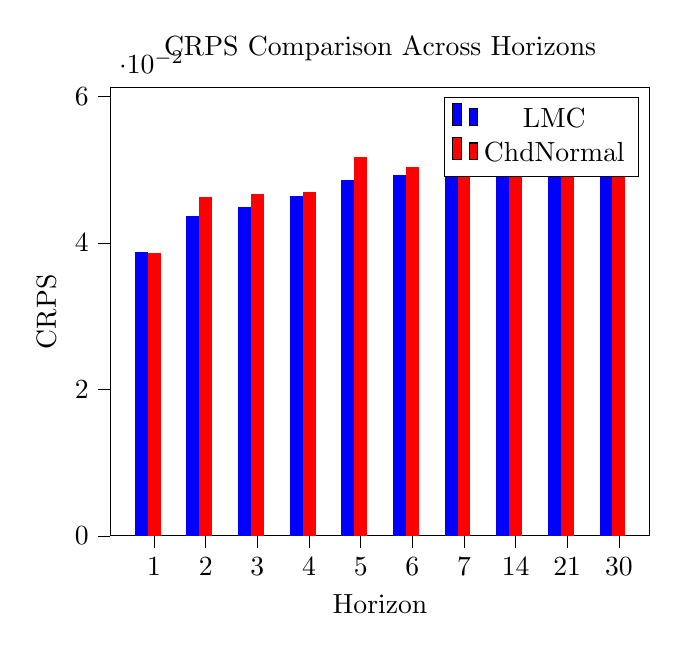
\begin{tikzpicture}

\definecolor{darkgray176}{RGB}{176,176,176}

\begin{axis}[
tick align=outside,
tick pos=left,
title={CRPS Comparison Across Horizons},
x grid style={darkgray176},
xlabel={Horizon},
xmin=-0.85, xmax=9.6,
xtick style={color=black},
xtick={0,1,2,3,4,5,6,7,8,9},
xticklabels={1,2,3,4,5,6,7,14,21,30},
y grid style={darkgray176},
ylabel={CRPS},
ymin=0, ymax=0.0611880252610714,
ytick style={color=black}
]
\draw[draw=none,fill=blue] (axis cs:-0.375,0) rectangle (axis cs:-0.125,0.0387614383507878);
\addlegendimage{ybar,ybar legend,draw=none,fill=blue}
\addlegendentry{LMC}

\draw[draw=none,fill=blue] (axis cs:0.625,0) rectangle (axis cs:0.875,0.0436182818138245);
\draw[draw=none,fill=blue] (axis cs:1.625,0) rectangle (axis cs:1.875,0.0449218988613064);
\draw[draw=none,fill=blue] (axis cs:2.625,0) rectangle (axis cs:2.875,0.0463205896836897);
\draw[draw=none,fill=blue] (axis cs:3.625,0) rectangle (axis cs:3.875,0.0485997453578194);
\draw[draw=none,fill=blue] (axis cs:4.625,0) rectangle (axis cs:4.875,0.049298678228726);
\draw[draw=none,fill=blue] (axis cs:5.625,0) rectangle (axis cs:5.875,0.0493409092729093);
\draw[draw=none,fill=blue] (axis cs:6.625,0) rectangle (axis cs:6.875,0.0530400553498712);
\draw[draw=none,fill=blue] (axis cs:7.625,0) rectangle (axis cs:7.875,0.0563757060878646);
\draw[draw=none,fill=blue] (axis cs:8.625,0) rectangle (axis cs:8.875,0.058274309772449);
\draw[draw=none,fill=red] (axis cs:-0.125,0) rectangle (axis cs:0.125,0.0385928704596256);
\addlegendimage{ybar,ybar legend,draw=none,fill=red}
\addlegendentry{ChdNormal}

\draw[draw=none,fill=red] (axis cs:0.875,0) rectangle (axis cs:1.125,0.0462132374189618);
\draw[draw=none,fill=red] (axis cs:1.875,0) rectangle (axis cs:2.125,0.0466448065791876);
\draw[draw=none,fill=red] (axis cs:2.875,0) rectangle (axis cs:3.125,0.0469528952861427);
\draw[draw=none,fill=red] (axis cs:3.875,0) rectangle (axis cs:4.125,0.0517437050659513);
\draw[draw=none,fill=red] (axis cs:4.875,0) rectangle (axis cs:5.125,0.0504136328508434);
\draw[draw=none,fill=red] (axis cs:5.875,0) rectangle (axis cs:6.125,0.0509588479433701);
\draw[draw=none,fill=red] (axis cs:6.875,0) rectangle (axis cs:7.125,0.0532882841366525);
\draw[draw=none,fill=red] (axis cs:7.875,0) rectangle (axis cs:8.125,0.0548539507173035);
\draw[draw=none,fill=red] (axis cs:8.875,0) rectangle (axis cs:9.125,0.0570231377331999);
\end{axis}

\end{tikzpicture}
